\documentclass[]{article}
\usepackage{float}
\usepackage{graphicx}
\usepackage[]{subcaption}
\captionsetup[figure]{labelfont={bf,footnotesize},textfont=footnotesize}
\captionsetup[table]{labelfont={bf,footnotesize},textfont=footnotesize}
\usepackage{xcolor}
\usepackage{listings}
\lstset{
  frame=single,
  breaklines=true,
  postbreak=\raisebox{0ex}[0ex][0ex]{\ensuremath{\color{red}\hookrightarrow\space}}
}
\usepackage{hyperref}

\newcommand{\TwoRowCell}[2][c]{%
\begin{tabular}[#1]{@{}c@{}}#2\end{tabular}}

\title{Simulation - Assignment 1}
\author{Anton Roth}
\date{\today}

\begin{document}
\begin{titlepage}
  \maketitle
  \thispagestyle{empty}
\end{titlepage}

\section{Task 1}
The system with two queues was implemented with the {\it Event-Scheduling} approach. The states for the system were; Length of Q2, number of arrivals to Q1 and number of rejected arrivals to Q1. Four events were implemented: Arrival to Q1, Departure of Q1 (combined with arrival to Q2), Departure of Q2 and Measure.

As model verifications the following was controlled numerically and graphically:
\begin{itemize}
  \item Inter-arrival times $\rightarrow 0$ :
    \begin{itemize}
      \item Length of Q1 $\rightarrow 10$.
      \item Rejection ratio of Q1 $\rightarrow 1$.
    \end{itemize}
  \item Inter-arrival times $\rightarrow \infty$ :
    \begin{itemize}
      \item Length of Q1 $\rightarrow 0$.
      \item Rejection ratio of Q1 $\rightarrow 0$.
    \end{itemize}
\end{itemize}

Measurements were made with time-differences exponentially distributed with a mean of 5 s. 10000 measurements were taken. The results of task 1 is presented in Table \ref{tab:task1}.

\begin{table}[H]
  \centering
  \caption{Results of task 1. For the three different inter-arrival times the mean value and the corresponding standard deviation (StdDev) is presented for length of Q2 and the rejection ratio of Q1.}
  \label{tab:task1}
  \resizebox{\textwidth}{!}{% Important that this only covers the tabular!
  \begin{tabular}{|c|c|c|c|c|}
  \hline
  \TwoRowCell{\bf Inter-arrival \\ \bf times Q1 (s)} & \TwoRowCell{\bf Mean length \\ \bf Q2} & \TwoRowCell{\bf StdDev length \\ \bf Q2} & \TwoRowCell{\bf Mean rejection \\ \bf ratio Q1} & \TwoRowCell{\bf StdDev rejection \\ \bf ratio Q1} \\ \hline
  1                                   & 11                      & 13                        & 0.52                             & 0.02                              \\ \hline
  2                                   & 4.4                     & 3.0                       & 0.070                            & 0.009                             \\ \hline
  5                                   & 0.43                    & 0.55                      & 0                                & 0                                 \\ \hline
  \end{tabular}%
}
\end{table}

From the results of length Q2 presented in Table \ref{tab:task1}, as the uncertainties is of the same order as the mean, the system state varies a lot. The rejection ratios are more significant and shows an expected behaviour, i.e. the shorter inter-arrival time the higher rejection rate.


\section{Task 2}
The {\it Event-Scheduling} approach was also used in this task and the code written for task 1 was used as a template.
The event structure was changed and a specific method was implemented for the addition of a job to the buffer.
The following events were used: AddJobA, AddJobB, ServeJobA, ServeJobB and Measure.
The states were simply the number of jobs of type A, denoted $NA$ and B, denoted $NB$, in the buffer.
Due to bad planning, an ugly solution was implemented for the case of adding a job from the buffer to serve (see code).

As a verification step the following was controlled:
\begin{itemize}
  \item Delay times $\rightarrow \infty$ :
    \begin{itemize}
      \item $NA + NB \rightarrow 0$. This is due to that the serve time of A, $x_A = 0.002$ s is shorter than the average arrival time $ \sim 0.0067$.
    \end{itemize}
  \item Serve time for job A and B $x_A, x_B \rightarrow \infty$ :
    \begin{itemize}
      \item $ NA + NB \rightarrow \infty$.
    \end{itemize}
\end{itemize}


\begin{table}[H]
  \centering
  \caption{Results of task 2 for the first three questions/simulation runs presented in the task description. For all runs the mean and standard deviation (StdDev) of the buffer length is presented.}
  \label{tab:task2}
  %\resizebox{\textwidth}{!}{% Important that this only covers the tabular!
  \begin{tabular}{|c|c|c|}
  \hline
  \textbf{``Run''} & \TwoRowCell{\bf Mean length \\ \bf of buffer} & \TwoRowCell{\bf StdDev length \\ \bf of buffer} \\ \hline
  1                                   & 130                      & 100            \\ \hline
  2                                   & 7.2                    & 7.9          \\ \hline
  3                                   & 3.6                     & 3.8           \\ \hline
  \end{tabular}%
%}
\end{table}

The simulation results is presented graphically in Figure \ref{fig:task2}.

\begin{figure}[H]
  \centering
  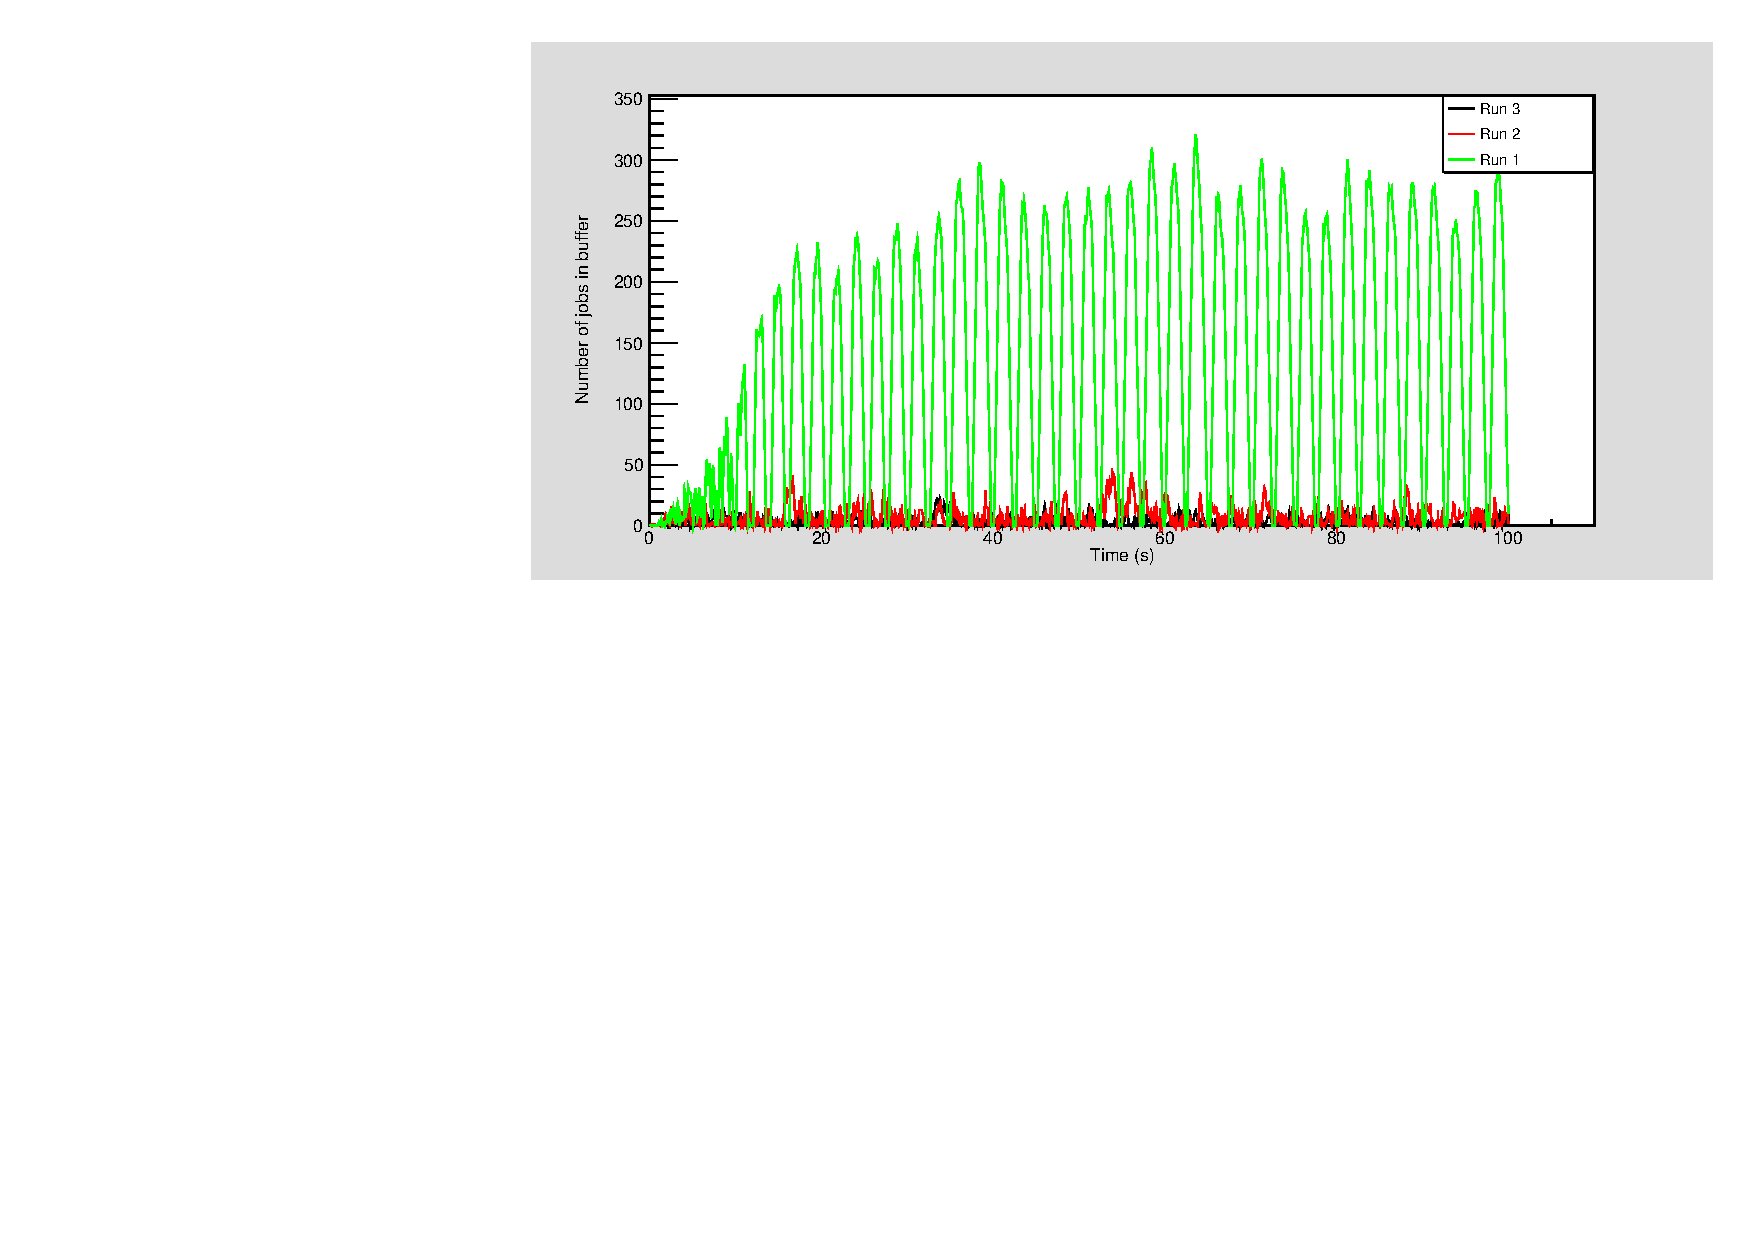
\includegraphics[width=\textwidth]{task2.pdf}
  \caption{Result of task 2. The number of jobs in the buffer as a function of the simulation time for the three runs (indicated in the legend).}
  \label{fig:task2}
\end{figure}

The result of run 1 and 2 differs substantially.
As job B is prioritised and feeded to a system with a delay of 1 s one obtains a periodicity.
Consider a constant delay of 1 s and the situation when the system starts up, the periodic behaviour can be explained with the following chain of events:
\begin{enumerate}
  \item Job A:s are added to the buffer and served efficiently. The buffer length is kept minimal.
  \item After 1 s job B:s are added to the buffer and since they are prioritised they are served immediately. The serving time is $ x_B > x_A $ and together with the fact that A jobs are continuously added to the buffer this implies that the buffer length will increase.
  \item After some time all B jobs have been served and A jobs are again served. The buffer length decreases.
  \item $\rightarrow$ point 2.
\end{enumerate}
Run 2 exhibits a weaker periodic behaviour since delay is now sampled from an exponential distribution.
This has the effect that all B jobs will not arrive at the server at the same time and the buffer length will not increase as much.

The mean length of the buffer for the third run is the lowest.
The buffer length no longer shows a clear periodic behaviour.
As type A jobs now are prioritised and have a shorter serving time, the buffer length can efficiently be kept at a minimal.
When there are no A jobs, B jobs which have a longer serving time will be processed.
The pile-up in the buffer is not possible due to the efficient processing of the jobs.

It should also be mentioned that there is a ``start-up'' period needed for the first run (although not implemented), as it takes some time for the buffer to stabilise in its periodic behaviour.
\section{Task 3}
A similar system compared to in task 1 was implemented.
One difference was the measure of the mean time a customer spends in the system.
The time spent by every customer in the system was stored in a container and used to calculate the mean.
Hence, it was not ``Measured'' as an event as this was considered the most efficient implementation and is not very computationally costly for the simulation.

Measurements were made with time-differences exponentially distributed with a mean of 5 s.
10000 measurements were taken.
The results of task 3 is presented in Table \ref{tab:task3}.

\begin{table}[H]
  \centering
  \caption{Results of task 3. For the three different mean arrival times the mean customer length and the mean queueing time for the simulation and analytical calculations are presented.}
  \label{tab:task3}
  \resizebox{\textwidth}{!}{% Important that this only covers the tabular!
  \begin{tabular}{|c|c|c|c|c|}
  \hline
  \TwoRowCell{\bf Mean arrival \\ \bf times (s)} & \TwoRowCell{\bf Mean customer \\ \bf length (simulated) } & \TwoRowCell{\bf Mean customer \\ \bf length (analytically) }& \TwoRowCell{\bf Mean queueing \\ \bf time (simulated) } & \TwoRowCell{\bf Mean queueing \\ \bf time (analytically) } \\ \hline
  2                                   & 1.98                      & 2                        & 3.99                             & 4                              \\ \hline
  1.5                                   & 4.02                     & 4                       & 5.99                            & 6                             \\ \hline
  1.1                                   & 18.5                    & 20                      & 20.2                                & 22                                 \\ \hline
  \end{tabular}%
}
\end{table}

The simulated values are very congruent with the analytical calculations in case of 2 and 1.5 s mean arrival times.
For the 1.1 s mean arrival time the simulated values deviate more from the analytical value.
The reason to why, is unclear.
A delayed start-up of 1000 s, chosen on the basis of the graphic evolution of the mean customer length, was tried but resulted in similar values.

\section{Task 4}
Task 4 was also solved with the {\it Event-Scheduling} approach and a similar implementation as in task 1.
Three events were defined; Arrival, Depart and Measure.
One system state was implemented as the number of customers, denoted $NC$,  in the system.

As model verifications the following was controlled numerically and graphically:
\begin{itemize}
  \item $ x \rightarrow 0$ : $ NC \rightarrow 0$
  \item $\lambda \rightarrow \infty$ : $ NC \rightarrow N$
\end{itemize}

\subsection{Question 1, 2 \& 3}
The simulation measurements for the settings in questions 1, 2 and 3 is presented in Figure \ref{fig:task4}.

\begin{figure}[H]
  \centering
  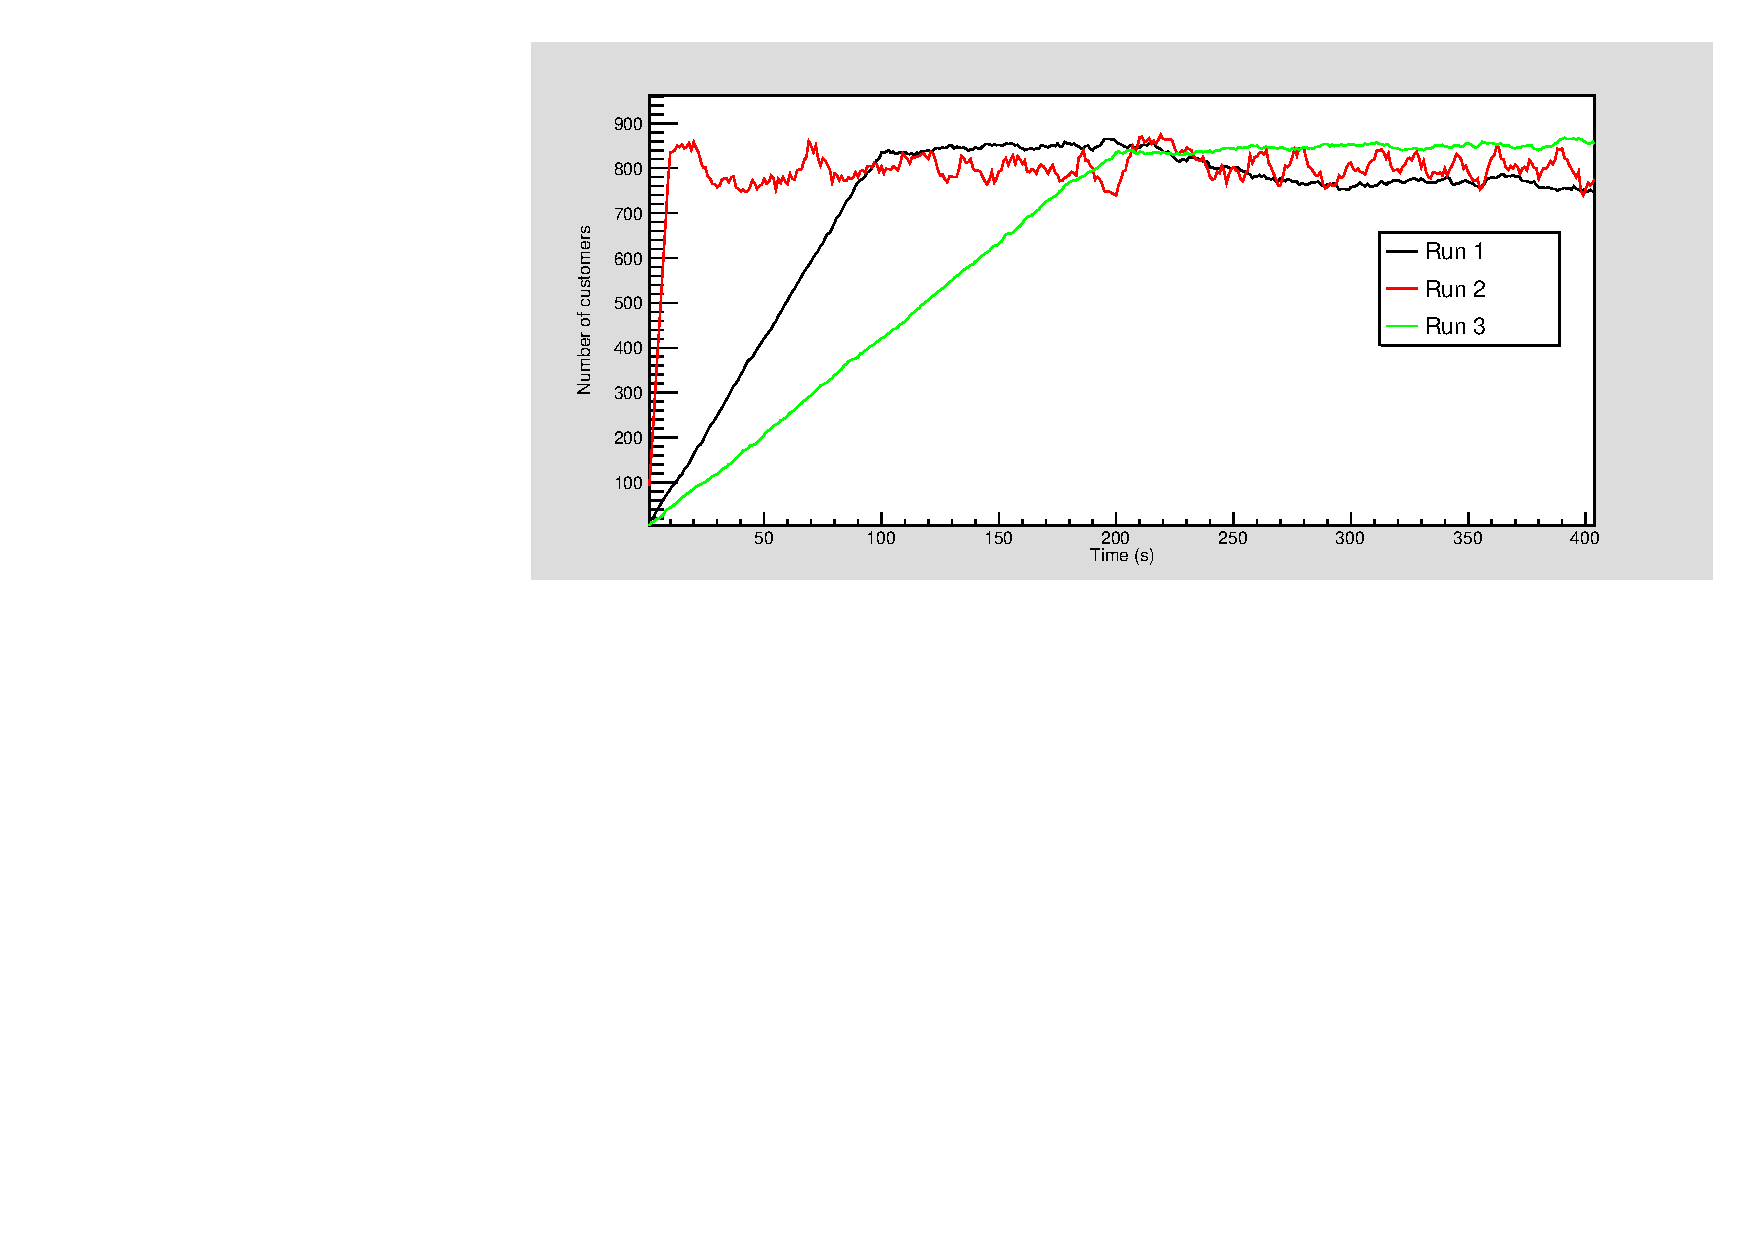
\includegraphics[width=\textwidth]{task4a.pdf}
  \caption{The number of customers as a function of simulation time is presented for the first three runs (indicated in the legend). The difference in length of the transient phase can be distinguished. }
  \label{fig:task4}
\end{figure}

Clear from Figure \ref{fig:task4} are different transient phases, i.e. time it takes till the system reaches an equilibrium in the total number of customers.
Reading out when the measurements plane out the length of the transient phases are obtained and this is presented in Table \ref{tab:task4a}.

\begin{table}[H]
  \centering
  \caption{Length of the transient phases for task 4 and the first three questions/simulation runs.}
  \label{tab:task4a}
  \begin{tabular}{|c|c|}
  \hline
  \textbf{``Run''} & \TwoRowCell{\bf Length of \\ \bf transient phase (s)} \\ \hline
  1 ($x = 100, \lambda = 8$)                                  & 100     \\ \hline
  2 ($x = 10, \lambda = 80$)                                 & 10 \\ \hline
  3 ($x = 200, \lambda = 4$)                                 & 200   \\ \hline
  \end{tabular}
\end{table}

For these three runs the number of customers in equilibrium is the same according to Little's theorem $ NC = \lambda \cdot x = 800$.
The parameter that governs the length of transient phase is the rate of arrivals to the system, $\lambda$.
The time it takes for the system to reach this number (assuming $ x >> \frac{1}{\lambda}$) is: $ t = \frac{800}{\lambda} $.

\subsection{Question 4, 5 \& 6}
The confidence interval is calculated using the provided {\it MATLAB} program.
In this program the system measurements are modeled as an auto-regressive process to compensate for the covariance contribution.
I consider this important for the current system since in a queue a future length is always highly dependent on the current and past queue lengths.
The effect on the variance from the correlation was checked with a comparison of equidistant and exponentially distributed measurement times.
The covariance contribution could be observed, i.e. the computed variance with the equidistant measurement times was lower.

The length of the 95\% confidence interval for the three different runs are presented in Table \ref{tab:task4b}.
\begin{table}[H]
  \centering
  \caption{Length of the 95\% confidence interval for task 4 and the last three questions/simulation runs.}
  \label{tab:task4b}
  \begin{tabular}{|c|c|}
  \hline
  \textbf{``Run''} & \TwoRowCell{\bf Length of \\ \bf 95\% confidence interval.} \\ \hline
  4 ($T = 4, M = 1000$)                                  & 1.17     \\ \hline
  5 ($T = 1, M = 4000$)                                 & 1.27 \\ \hline
  6 ($T = 4, M = 4000$)                                 & 0.64 \\ \hline
  \end{tabular}
\end{table}

%Period of arrivals: $\frac{1}{\lambda} = 0.25$s.

What is very interesting from the result presented in Table \ref{tab:task4b} is that the confidence interval for run 5 is longer than that of run 4 even though the number of measurements is larger in the fifth run.
The {\it MATLAB} modeled AR-process needs several more parameters, cf. an AR-order of 23 for run 5 and 2 for run 4.
This indicates that run 5 contains a lot more information than run 4 and this is reasonable due to the 3000 more samples.
My hypothesis is that run 5 catches a short periodic behaviour which run 4 does not and in turn increases the variance.
The confidence intervals were also calculated for exponentially distributed measurement times and the following results were then obtained:
\begin{table}[H]
  \centering
  %\caption{Length of the 95\% confidence interval for task 4 and the last three questions/simulation runs.}
  %\label{tab:task4b}
  \begin{tabular}{|c|c|}
  \hline
  \textbf{``Run''} & \TwoRowCell{\bf Length of \\ \bf 95\% confidence interval.} \\ \hline
  4 ($\exp(T = 4), M = 1000$)                                  & 2.17     \\ \hline
  5 ($\exp(T = 1), M = 4000$)                                 & 1.57 \\ \hline
  6 ($\exp(T = 4), M = 4000$)                                 & 1.00 \\ \hline
  \end{tabular}
\end{table}
The results presented above strengthens the hypothesis, since the periodicity in the samples should be suppressed with exponentially distributed measurements.

Run 6 has the optimal (as far as it concerns the above measurements) settings.
A time of 4 s between each measurement seems to smoothen out the data and the many measurements shrinks the confidence interval, as it should.

\section{Task 5}
The system in this task was implemented with the {\it Process Interaction} method.
It took quite some time to get it right.

Three different processes, i.e. classes, were implemented; Generator, Queue and Measure.
The interaction between the processes was implemented with a Signal class which comprised a SignalType, a receiving process Destination, and ArrivalTime, plus an optional parameter representing the measured values sent to the Measure process.
A helper class ProcessList holds all Processes and controlls the Signal which is to be treated.
A base class LoadDistr with derived classes RandomLoad, RobinLoad and SmallestQue were also implemented.
The Generator process possesses an object of type LoadDistr which has a function GetQ which is invoked when Queue is chosen.

The system was first tried on just one Queue and verified with Little's theorem.
In this process it was noted that if the mean arrival time was smaller than the mean service time, the system diverged.
It was observed that for mean inter-arrival times $\rightarrow$ mean service time a mean queue length longer than the value from Little's theorem was always obtained.
However, for larger inter-arrival times the queue length agreed with Little's theorem.
Why this is the case is still unclear.
The chain of signals have been closely controlled and these work as they are intended.
The sampling from the uniform distribution and the exponential distribution has also been verified to work.

The system with all load distributions were then tried to be verified with a mean arrival time of 0.12 seconds.
However, the obtained mean number of jobs in the queuing system was not congruent with Little's theorem in this case.
It was assumed that

\begin{table}[H]
  \centering
  \caption{Results of task 5. For the three different inter-arrival times the mean value $\pm$ its standard deviation is presented for all load distributions and mean arrival times.}
  \label{tab:task5}
  \resizebox{\textwidth}{!}{% Important that this only covers the tabular!
  \begin{tabular}{|c|c|c|c|}
  \hline
  \TwoRowCell{\bf Inter-arrival \\ \bf times (s)} & \TwoRowCell{\bf Random load \\ \bf distribution} & \TwoRowCell{\bf Robin load \\ \bf distribution} & \TwoRowCell{\bf Smallest queue \\ \bf distribution}  \\ \hline
  0.11                                   & 11                      & 13                        & 0.52                                                       \\ \hline
  0.15                                   & 4.4                     & 3.0                       & 0.070                                                      \\ \hline
  2                                   & 0.43                    & 0.55                      & 0                                                          \\ \hline
  \end{tabular}%
}
\end{table}


\section{Task 6}
The system was implemented with a simplified {\it Event-Scheduling} approach.
Two events; Arrival and Depart was implemented.
The system state was the number of prescriptions to be filled in.
New arrivals were generated if the arrival time was before the closing time.
The stopping condition for a working day's simulation was an empty event list and 1000 days were simulated.
The event time of each day's last departure was measured and stored in a container.
The mean of the container elements was the average time his work will finish every day.
The time difference of the arrival and departure of each prescription was also stored in a container and used to calculate the average time it takes to fill a prescription.
The results of task 6 is presented in Table \ref{tab:task6}.

\begin{table}[H]
  \centering
  \caption{Results of task 6. The average time the work finishes and the average time it takes to fill a prescription is presented with $\pm \sigma$ (standard deviation).}
  \begin{tabular}{c | c}
    Average time work finishes & Average time it takes to fill prescription \\ \hline
    17:24 $\pm 15$ & $25 \pm 11$ min
  \end{tabular}
  \label{tab:task6}
\end{table}

\section{Task 7}
The system in task 7 was implemented with a small scale {\it Event-Scheduling} approach.
First the life time for each of the components were generated and stored in an event list, then the event list was stepped through in chronological order and the time at which all components were ``dead'' was stored in a container.
The mean of this container, which is the average life time of the system, is the result presented in Table \ref{tab:task7}.
\begin{table}[H]
  \centering
  \caption{The result of task 7. The average life time is presented with its uncertainty (standard deviation).}
  \begin{tabular}{c}
    Average life time of the system \\ \hline
    $3.67 \pm 0.93$
  \end{tabular}
  \label{tab:task7}
\end{table}



\section*{Code}
Below the c++-code used for the assignement is presented. Header files and Makefiles have been left out. I would strongly recommend to study the source code in the attached .zip file instead of trying to read here.
Also, note that the framework ROOT [\url{https://root.cern.ch/}] has been used to visualise the data.

\subsection{Task 1}
{\large File: eventandstate.cc}
\lstinputlisting[language=c++]{../task1/eventandstate.cc}

{\large File: main.cc}
\lstinputlisting[language=c++]{../task1/main.cc}

\subsection{Task 2}
{\large File: eventandstate.cc}
\lstinputlisting[language=c++]{../task2/eventandstate.cc}

{\large File: main.cc}
\lstinputlisting[language=c++]{../task2/main.cc}

\subsection{Task 3}
{\large File: eventandstate.cc}
\lstinputlisting[language=c++]{../task3/eventandstate.cc}

{\large File: main.cc}
\lstinputlisting[language=c++]{../task3/main.cc}

\subsection{Task 4}
{\large File: eventandstate.cc}
\lstinputlisting[language=c++]{../task4/eventandstate.cc}

{\large File: main.cc}
\lstinputlisting[language=c++]{../task4/main.cc}

\subsection{Task 5}
{\large File: procs.cc}
\lstinputlisting[language=c++]{../task5/procs.cc}

{\large File: main.cc}
\lstinputlisting[language=c++]{../task5/main.cc}

\subsection{Task 6}
{\large File: eventandstate.cc}
\lstinputlisting[language=c++]{../task6/eventandstate.cc}

{\large File: main.cc}
\lstinputlisting[language=c++]{../task6/main.cc}

\subsection{Task 7}
{\large File: main.cc}
\lstinputlisting[language=c++]{../task7/main.cc}


 \end{document}
